\chapter{相关概念及研究}
\label{ch2}

本章首先介绍了智能网联汽车的网络系统架构,包括 TSP 云服务、V2X 车载通信等分别分析了它们的
系统架构的组成和原理,其次还介绍了目前主要的攻击手段和智能网联汽车面临的主要威胁。
对目前主流威胁建模方法进行了介绍,最后还介绍了层次分析法为后续威胁模型的提出作前置理论准备。

\section{智能网联汽车联网系统架构}

\subsection{车载网络架构划分}
车载网络架构如图2.1所示。这是一个
以域为中心的体系结构,具有以太网作为主干,分为五个领域:动力系统、底盘、车
身、信息娱乐和高级驾驶辅助系统(ADAS)。每个域控制
器通过一个中央网关与以太网主干连接。CAN/CAN FD 和
LIN 用作每个域中的通信协议。此外,车载网络可以通
过远程信息处理单元和接口(如 OBD、USB 和 Wi-Fi)连接
到外部网络。这种集中式架构通过域控制器和以太网提
供智能网联汽车所需的计算和通信能力。然而,车辆的外部接
口也增加了。这些开放的接口给智能网联汽车带来了新的攻击
面和安全隐患。
\begin{figure}
  \centering
  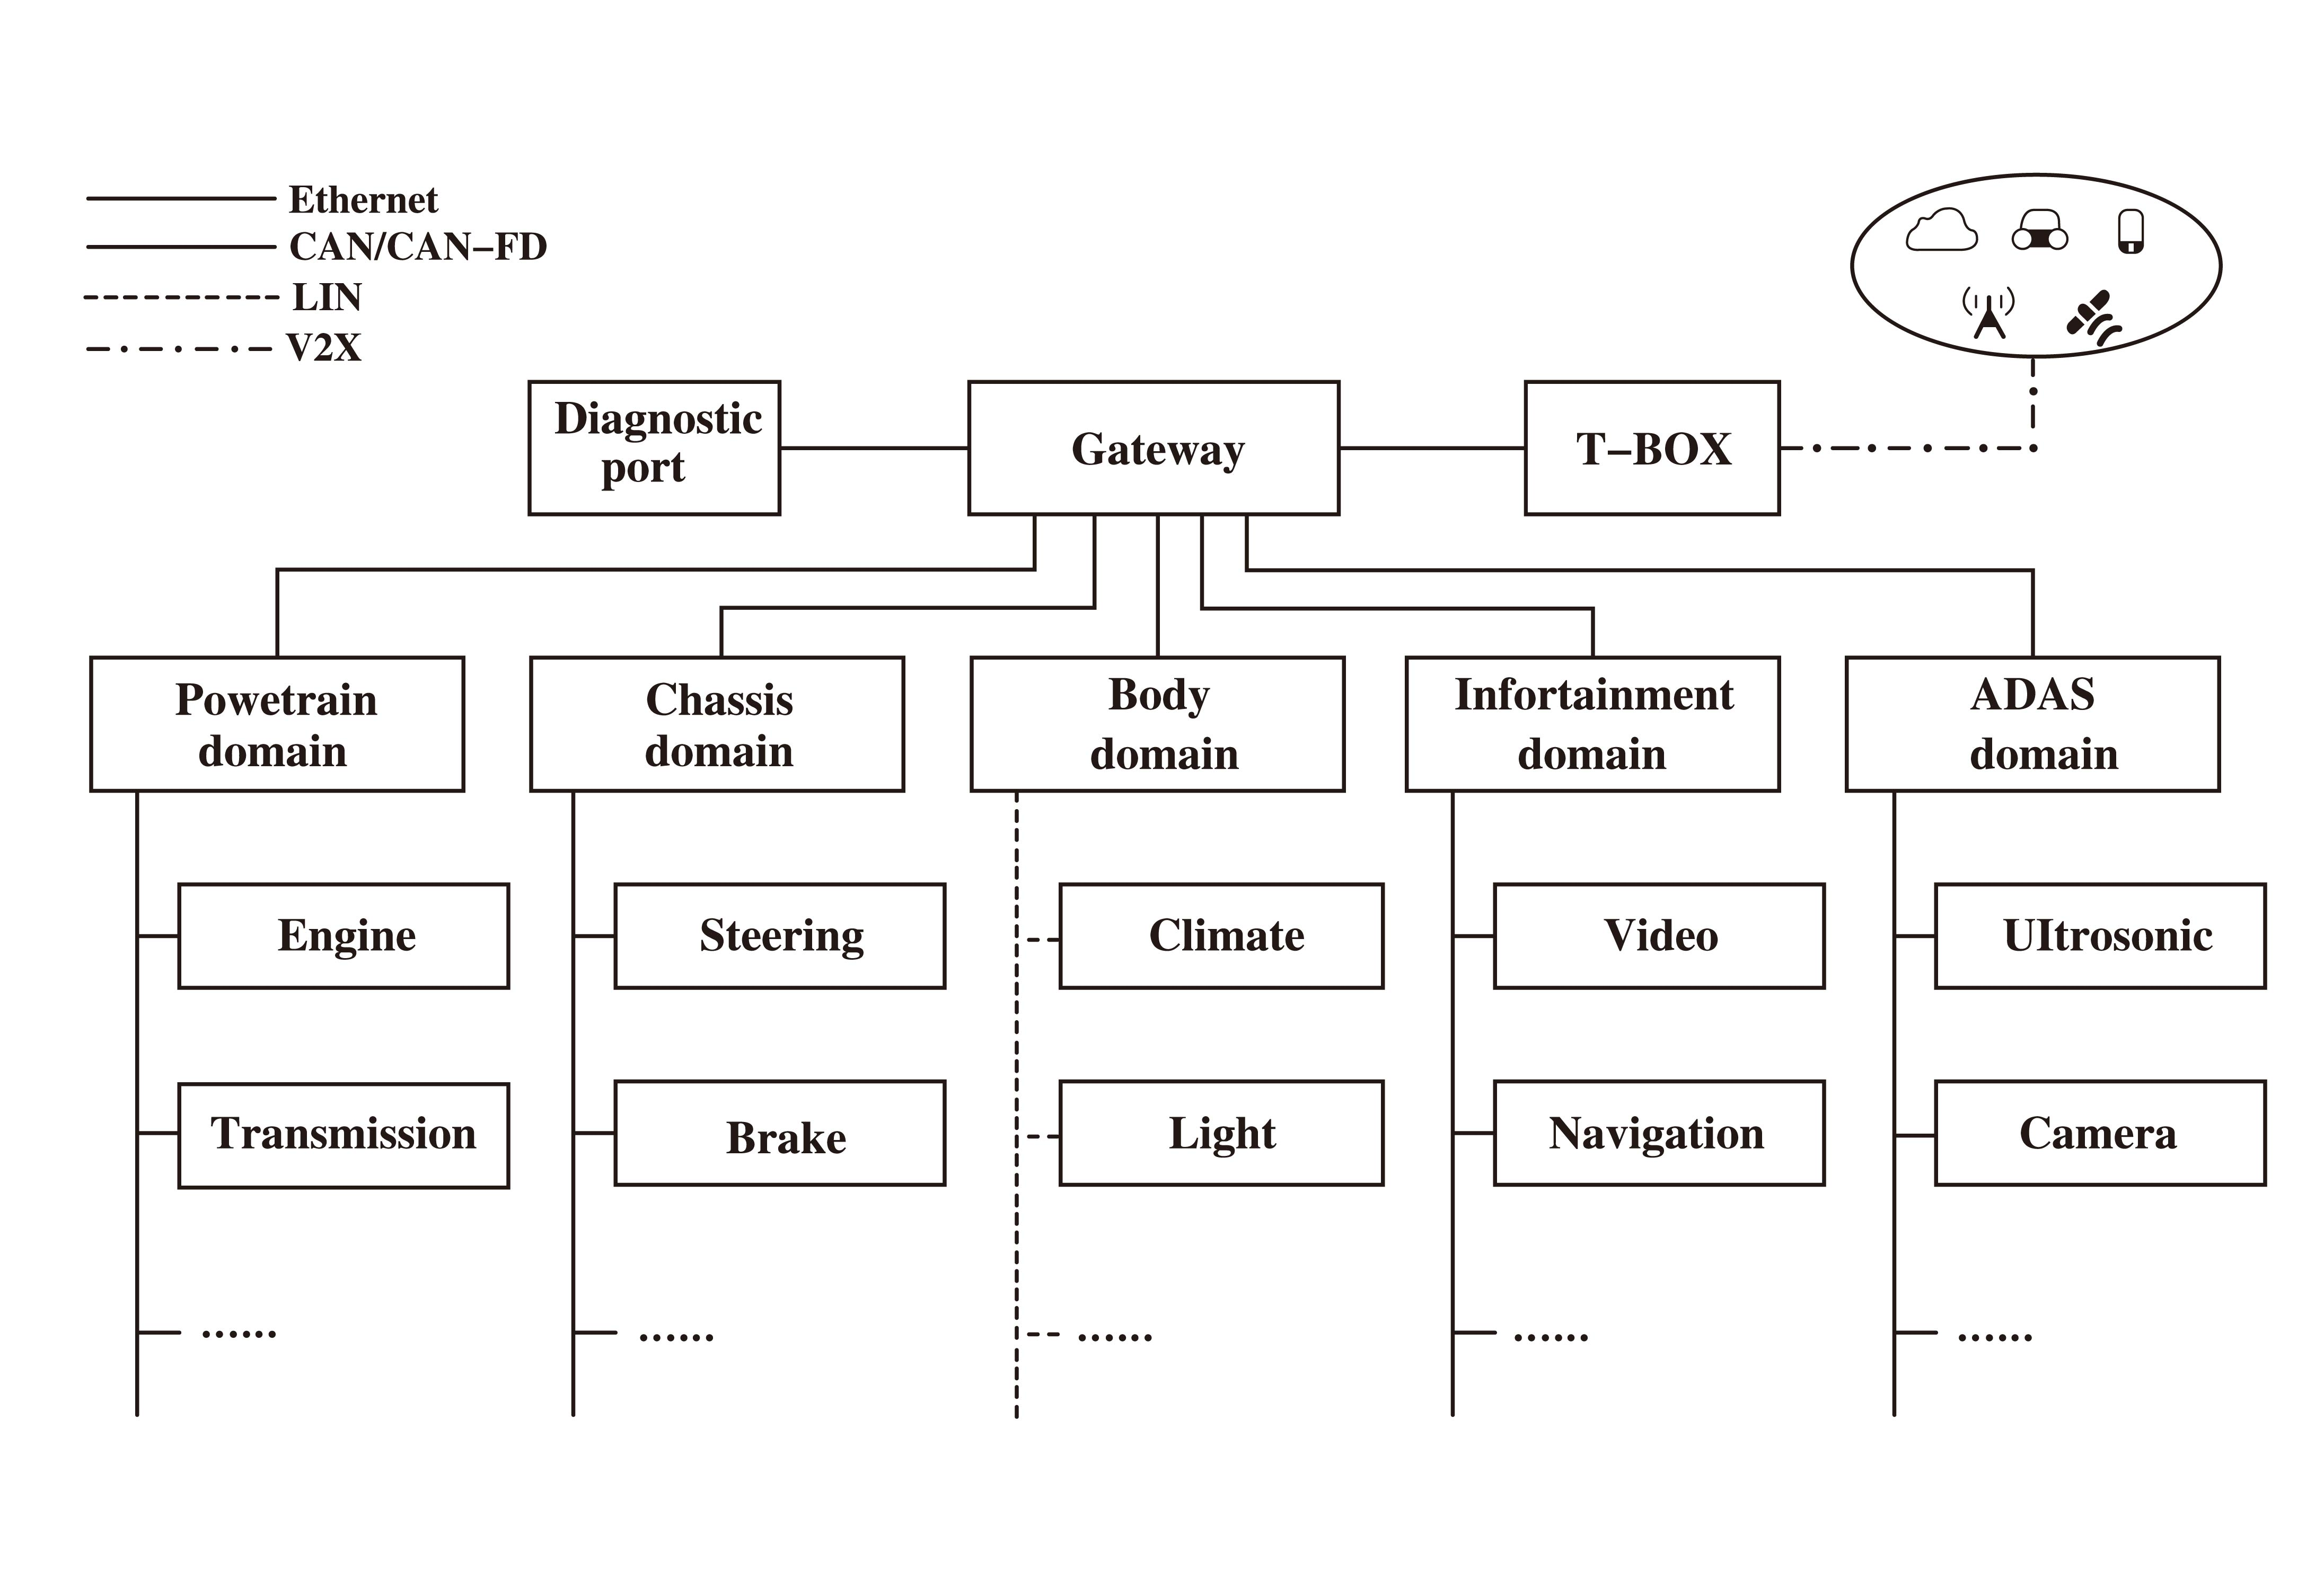
\includegraphics[scale=0.4]{resources/img/i1.jpg}
  \caption{车联网网络架构图}
\end{figure}
目前的汽车结构中,车辆内部网络主要由 CAN
总线和 ECU 组成。ECU 是嵌入式设备,包括各种智能系统,如紧急制动辅助
(EBA,electronic brake assist)、防抱死制动系统(ABS,
antilock brake system)等。CAN总线是 ECU间的接口
能把汽车里的 ECU 连接在一起的通讯桥,
使它们能够进行高效的信息通信。

智能网联汽车中的 CAN 总线与众多嵌入式设备的多功能连接,为用户提供了方便,但也存在着易被入侵的问题。黑客能够利用车载信
息娱乐(IVI,in-vehicle infotainment)系统暴露出来的外部接口如USB等恶意进入系统内部获取隐私信息。

车载诊断界面主要用于车辆故障的检测和废气监测,而OBD-II接口则一般是非法侵入车辆 CAN总线数据的通道。另外,T-BOX,胎压。
许多嵌入式设备如 TPMS、 RKE、 ABS等都有大量可利用的攻击面。

这里简单的介绍上述英文名词的定义。
\begin{itemize}
    \item CAN 控制器局域网(Controller Area Network,简称CAN或者CAN bus) CAN 总线是一种基于消息的协议,旨在允许当今汽车以及其他设备中的电子控制单元 (ECU) 以可靠的、优先级驱动的方式相互通信。网络中的所有设备都可以接收消息或“帧”,这不需要主机。CAN 受到ISO-11898下的一组丰富的国际标准的支持。
    \item ADAS 可帮助驾驶员进行驾驶和停车功能。通过安全的人机界面,ADAS 提高了汽车和道路的安全性。ADAS 使用传感器和摄像头等自动化技术来检测附近的障碍物或驾驶员错误,并做出相应的反应。ADAS 可以实现不同级别的自动驾驶,具体取决于车内安装的功能。
    \item OBD是英文On-Board Diagnostics的缩写,是智能网联汽车内部的计算机系统,用于跟踪和调节汽车的性能。该车载计算机系统从车辆内部的传感器网络收集信息,然后系统可以使用这些信息来调节汽车系统或提醒用户注意问题。技术人员可以简单地插入 OBD 系统以收集车辆数据并诊断问题。OBD 系统在帮助用户更好地了解车辆诊断方面提供了很大帮助。
    \item ECU(Electronic Control Unit)电子控制器单元,又称为汽车的“行车电脑”,是车辆内部的一种小型设备,用于控制该车辆中的一个或多个电气系统。它告诉电气系统该做什么以及如何操作。ECU的核心是一个微控制器,由嵌入式软件控制。它们的用途就是控制汽车的行驶状态以及实现其各种功能。它主要是利用各种传感器和总线进行数据的收集和交换,从而判断出驾驶员的驾驶意图和驾驶意图,并由执行器控制汽车。
    \item T-BOX作为无线网关,是远程信息处理控制单元(TCU),由GPS单元、通信外部接口、电子处理单元、微控制器、移动通信单元和内存组成,实现车内终端信息的交互、云和路边单元(RSU)。一般具有故障诊断、低功耗设计、休眠唤醒、SD卡扩展、输出电源、RS232/485、USB和IO接口等新功能。
\end{itemize}
\subsection{TSP 云端通信技术}

(Telematics Service Provider)汽车远程服务提供商,在Telematics产业链居于核心地位,上接汽车、车载设备制造商、网络运营商,下接内容提供商。
 Telematics结合了GPS系统、车载车辆诊断、无线远程信息处理设备和黑匣子技术,以记录和传输车辆数据,如速度、位置、维护要求和服务,并将这些数据与车辆的内部行为进行交叉引用。这些信息可用于实时分析,以提高整体驾驶员安全,降低成本并提高商用车辆的性能。
 \begin{figure}
    \centering
    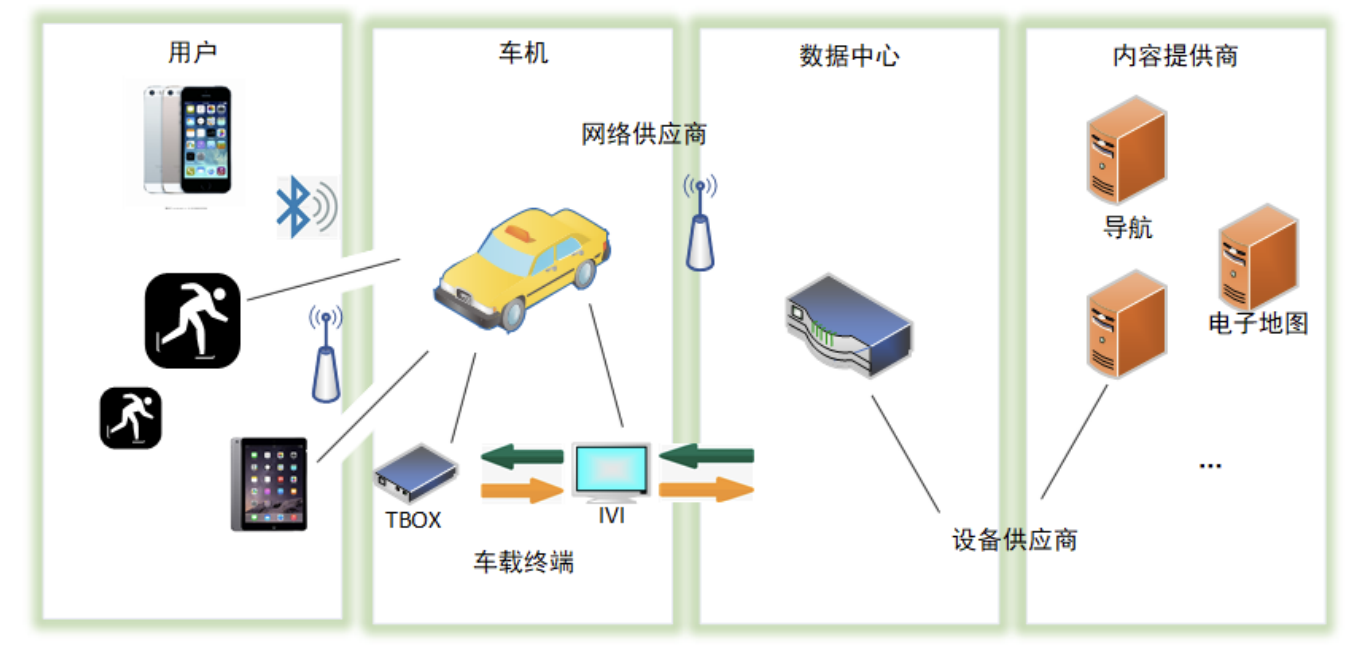
\includegraphics[scale=0.6]{resources/img/i2.png}
    \caption{TSP 系统组成}
  \end{figure}

  远程信息处理系统通常具有以下组件:
  \begin{itemize}
    \item 车队通信软件系统
    \item GPS跟踪设备
    \item 引擎接口
    \item 输入/输出接口
    \item SIM卡
    \item 加速度计
    \item 蜂鸣器
  \end{itemize}

Telematics目前主要应用在车载系统上,根据使用目的不同,Telematics可分为三种基本类型,即交通信息与导航服务、安全驾驶与车辆保护及故障诊断的车辆维护服务、娱乐及通信服务。提供全球定位系统技术、地理信息系统、智能型交通系统技术。值得一题的是Telematics逐渐演变为综合了GPS的跟踪装置和无线通信等技术的车载系统。

TSP一词狭义的在互联汽车行业中被用作
对服务提供者进行分类的广义术语
以安全车到云为核心的汽车价值链
数据管理。然而,目前TSP扮演的传统角色
在价值链中不断进化。TSP一词已被
IT公司,系统集成商,甚至一级企业等采用。网络
运营商正在将其M2M/IOT服务扩展到
汽车行业,意图将数据连接“去商品化”。
越来越多的汽车制造商通过TSP创造和集成更多的车载部件。

\subsection{V2X 车载通信技术}

Vehicle to Everything (V2X) 是一种车载通信系统,支持将信息从车辆传输到可能影响车辆的交通系统的移动部件。V2X 技术的主要目的是提高道路安全、节能和道路交通效率。

车联网的工作原理: 在 V2X 通信系统中,信息通过高带宽、高可靠性的链路从车辆传感器和其他来源传播,使其能够与其他汽车、停车位和交通信号灯等基础设施以及使用智能手机的行人进行通信。
通过与车辆周围的其他实体共享速度等信息,该技术提高了驾驶员对潜在危险的认识,并有助于降低伤害、道路事故死亡和与其他车辆碰撞的严重程度。
该技术还通过警告驾驶员即将到来的交通、建议替代路线以避免交通和识别可用停车位来提高交通效率。

V2X 技术的组成部分:
V2X技术的关键组成部分包括V2V(车对车)和V2I(车对基础设施)。V2V 允许车辆与道路上的其他车辆进行通信,而 V2I 允许车辆与外部实体进行通信,例如交通信号灯、停车位、骑自行车的人和行人。这些技术有助于改善道路安全、减少燃料消耗并增强驾驶员与其他道路使用者(例如骑自行车者和行人)之间的体验。

当 V2X 系统集成到传统车辆中时,驾驶员可以接收有关天气模式、附近事故、道路状况、道路工程警告、紧急车辆接近以及使用同一条道路的其他驾驶员活动的重要信息。

配备 V2X 系统的自动驾驶汽车可以为车辆现有的导航系统提供更多信息。该系统还使自动驾驶汽车能够扫描周围环境并根据收到的信息立即做出决定。
\begin{figure}
    \centering
    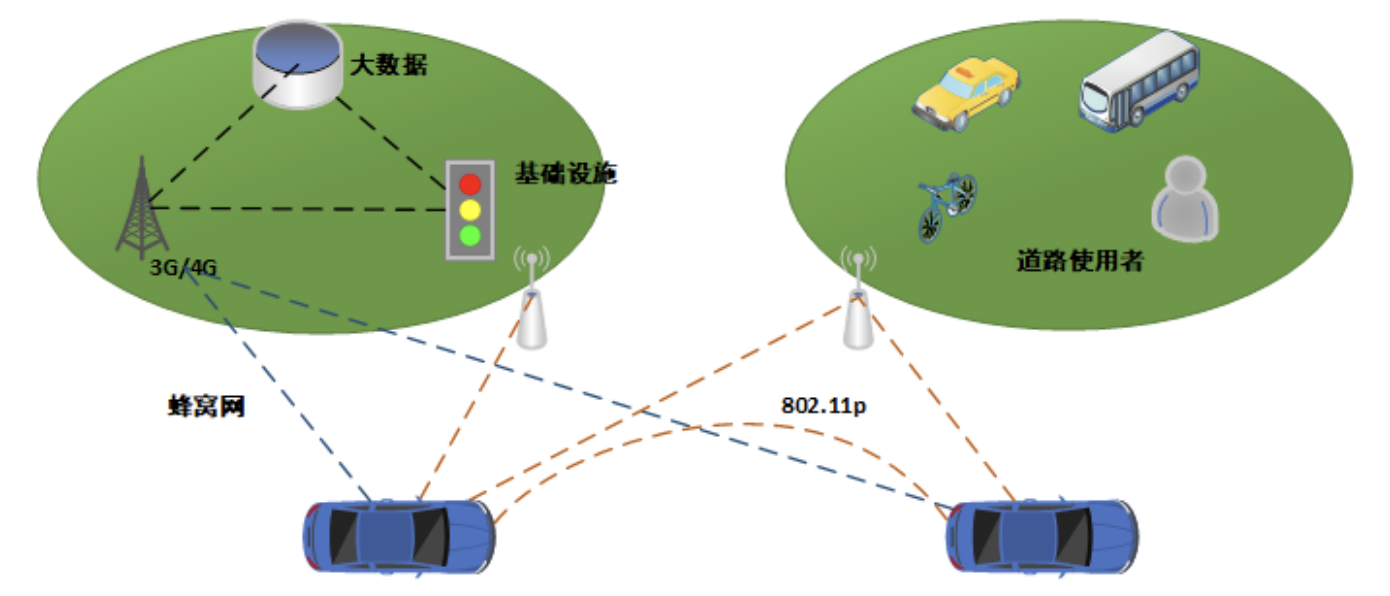
\includegraphics[scale=0.6]{resources/img/i3.png}
    \caption{v2x 应用场景}
  \end{figure}
\newline
如图2.3所示,是基于 V2X 简单的一个应用场景。智能网联汽车不仅可以借
助蜂窝网络,使得汽车与基站、云平台、路边单元等基础设备相连接实现 V2I,
而且还可以通过基站,与周围的车辆进行连接,从而实现 V2V。智能网联汽车在
与其他基础设备、非机动车、车辆、行人等进行通信的时候,使用诸如 802.11p
等协议。

\section{智能网联汽车主要攻击手段}
发明车载网络协议时,安全问题并不是主要问题。因此,许多安全功能天生就缺失了。例如,CAN 缺乏必要的保护来确保信号的可用性、机密性和真实性\cite{woo2014practical}。
FlexRay 虽然能够在出现错误的情况下保持正确操作,但无法抵御格式良好的恶意错误消息\cite{kleberger2011security}。尽管如此,这些缺点在过去并未构成迫在眉睫的安全威胁,因为车辆很少与外界连接,
而老式的安全攻击通常需要对车载网络进行物理访问。

然而,现代车辆正在通过各种方式迅速变得更加互联,用于许多高级应用。例如,车辆可以通过 DSRC(专用短程通信)连接以实现 VANET(车载自组织网络)功能,
通过 Wi-Fi/蓝牙实现车载娱乐,并通过蜂窝网络实现远程信息处理服务。尽管这些连接使车辆更加智能和舒适,但它们也将车载网络大量暴露给外部对手。
例如,CAN 通信可能会被智能手机恶意软件通过蜂窝网络远程篡改\cite{woo2014practical}。软件病毒可能通过受感染的娱乐媒体(如 CD(光盘)或蓝牙播放器)传播到车载组件。
此外,还可以通过攻击OEM存储中心的ECU密钥管理不善来侵入车载网络。

此外,直接访问的威胁仍然存在,因为攻击者也可能物理侵入通信线路,直接针对网络组件的弱点发起攻击。这种典型的攻击可能包括反汇编可执行代码和将恶意代码注入运行时环境。

车载网络的安全漏洞不仅可能对车辆用户造成严重后果,还会对其他道路交通参与者造成严重后果。例如,安全漏洞可能导致车辆用户的隐私泄露。目标私人数据可能包括车辆诊断流
、机柜对话、摄像记录、驾驶模式和车辆位置\cite{amoozadeh2015security}. 
这种典型的攻击是通过未经授权的窃听进行的。其次,安全漏洞可能导致车主或原始设备制造商的直接金钱损失。在此类攻击中,
攻击者经常故意修改或重放所需的车载数据以实现非法收益,例如车辆盗窃或里程表欺诈。第三级安全漏洞可能会对车辆使用者造成安全威胁。
这种攻击通常涉及对安全关键车载数据的恶意修改或伪造,例如轮胎压力、车速、发动机扭矩请求和制动命令. 
这可能导致非自愿驾驶机动甚至交通事故。考虑到自动驾驶的出现,这种危险至关重要,值得研究界更多关注。
第四,车载网络安全漏洞会对其他道路参与者造成安全威胁,甚至瘫痪整个交通系统。由于车辆将在大型网络中互连,
例如 VANET,因此信号可信度对于协调交通系统中的所有车辆都极为重要\cite{harding2014vehicle}.
 但是,如果车载网络安全受到损害,这种可信度可能会被破坏。
 例如,被篡改的车载网络可能会产生虚假数据,如果虚假数据已经传播到车辆外部并被其他人认为是“值得信赖的”,则可能对其他车辆造成极大的危险。
综合上述研究现状,将攻击手段分为以下类型:
\begin{itemize}
    \item 远距离通信攻击: 如利用蜂窝网络、Wi-Fi等进行伪装拦截通信信号等从而达到攻击的目的。
    \item 近距离车外通信: 利用蓝牙攻击和高频无线电攻击。如通过蓝牙连接车载娱乐系统,伪装发送信号给车载娱乐系统从而达到攻击的目的。
    \item 车辆内部网络: 如通过车辆内部USB攻击IVI系统等。
\end{itemize}

\section{智能网联汽车面临的安全威胁}
安全性是智能网联汽车面临的迅速出现的重大挑战。在车载网络的背景下,安全问题通常是指通信数据可能被恶意攻击者窃听、欺骗、丢弃、修改、泛滥、窃取等危险情况。
在车辆向自动驾驶和协作驾驶发展的时代,安全性在车载网络的设计中变得越来越重要。

\subsection{ICV 中的潜在威胁}
在远距离通信中,恶意攻击者入侵汽车的方
式大体可以分成四类:蜂窝网络、Wi-Fi、车载单元
(OBU,on board unit)/路侧单元(RSU,road side
unit)和全球定位系统(GPS,global positioning
system)。

(1) 蜂窝网络
蜂窝网解决了 ICV的远程通讯问题,但也存在着一些新的安全问题。比如,
利用无线通讯通道进行汽车定位追踪及通讯监视。
破解汽车固件,可实现了车辆的遥控(如方向盘等)。


(2) Wi-Fi
黑客通过 Wi-Fi 连接可以进行很多恶意攻击。如利用 Wi-Fi 远程访问车内网络;入侵IVI系统安装木马;监控汽车通信管道和访问流量。在文献\cite{keen}中,腾讯科恩安全实
验室研究员远程入侵了特斯拉汽车的网关、BCM 和
自动驾驶系统。它还能实现特斯拉电动汽车的天窗和车门的遥控启动,以及在驾驶过程中制动
利用安全漏洞,远程入侵了特斯拉车的网络。
并且可以对特斯拉进行任意的车身和驾驶控制。

(3) GPS
GPS 是汽车导航中最重要部分。在无人
驾驶中,GPS 导航作为汽车的“大脑”,能够为汽
车提供最优的行车路径,从而确保 GPS系统的安全性。
这是一个在自动驾驶方面很有意义的工作。文献\cite{cuigai}
显示了使用便携 GPS诱骗装置对汽车 GPS进行了篡改,造成严重的破坏。

\subsection{近距离车外通信的潜在威胁}
在近距离车外通信中,恶意攻击者入侵汽车的
方式主要为蓝牙攻击和高频无线电攻击两类。

(1) 蓝牙攻击
Bluetooth是一种无线技术,它能在手机、 IVI等多种设备间进行无线通讯。攻击者可以从
通过 Bluetooth界面来实现对车辆 IVI系统的恶意木马植入,
从而实现了对汽车内部网络的渗透和侵入。文献\cite{antian}
基于 Bluetooth的漏洞,他们研发了一个叫做“BlueBorn”的攻击程序
通过蓝牙通讯实现了入侵IVI系统。

(2) 高频无线电攻击
文献\cite{wuxiandian}描述了使用无线电欺骗实现了对汽车 TPMS 系统的攻击。在RKE、无钥匙点火等电子元
件中高频无线电的使用吸引了研究者的关注,很多黑客开始通过无线电欺骗的方式攻击车内外近距离通信。

\subsection{车辆内部网络的潜在威胁}
车辆内部网络的攻击面大致可分为 USB 接口
和 CAN 接口两部分。

(1) USB 接口
在 ICV 系统中,USB 接口可以直接与 IVI 连接,实
现自动播放音频和视频文件的功能。因此,黑客
可以通过插入USB盘向车内植入木马病毒从而实现对汽车的控制。
2015 年,黑客曾利用 USB 攻击造成马自达汽车 IVI
系统瘫痪。

(2) CAN 接口
CAN总线作为 ECU间的通信信道,它与 CAN总线协同工作,可以实时监控汽车的运行状态,然而 CAN总线仍然有一定的缺点。现在,很多车辆都装有保险狗, Mobileye,ELM327等,这些设备可以向使用者发出车道偏离警告,前方碰撞警告,以及速度警告。攻击者可以通过无线网络向 CAN总线传送命令,让攻击方可以遥控汽车的状况。文献\cite{koscher2010experimental}利用侧信
道攻击,通过CAN总线采集数据通信来窃听驾驶
人员的个人隐私,证实ICV中存在用户的个人隐私信息
有被泄漏的危险。

\section{威胁建模方法论}
威胁建模被定义为根据业务和技术利益相关者的输入,主动识别和解决对组织系统的潜在威胁的过程。通常在设计产品或新功能时完成,以避免将来出现安全漏洞的成本。

威胁建模是分析系统的各种业务和技术要求、识别潜在威胁并记录这些威胁对系统的脆弱程度的过程。威胁是指未经授权的一方访问组织的敏感信息、应用程序或网络的任何情况。 
威胁建模过程的目的是清楚地了解组织的各种资产、对这些资产的可能威胁,以及如何以及何时可以减轻这些威胁。威胁建模的最终产品是一个强大的安全系统。 
2020 年 4 月,视频通讯应用 Zoom 的股价从 159.56 美元跌至 111.41 美元。一旦用户群增加,Zoom 的许多安全漏洞就会暴露出来——其中大部分是 Zoom 没有预料到的。
2020 年 7 月,Twitter 以一组具有内部系统访问权限的员工为目标而遭到黑客攻击,导致 当时通过比特币汇款的用户损失了 117,000 美元。 
有了这样的安全攻击,品牌就会失去资本和信任。恶意软件攻击事件不会很快停止。
Cyber​​security Ventures 预测\cite{apache1},到 2021 年,网络犯罪损失每年将给全世界造成约 6 万亿美元的损失。这正是威胁建模过程可以在很大程度上减轻这些风险的地方。 
\newline
举例来说,在智能网联汽车中手机APP存储用户信息的过时加密算法是威胁建模的一个应用。
\begin{itemize}
    \item 漏洞是MD5等过时的加密算法。
    \item 威胁是使用暴力破解散列密码。
    \item 攻击者是试图在线出售个人信息的黑客。
    \item 缓解策略是将加密算法更改为更现代和更强大的东西。
  \end{itemize}
威胁建模可以通过三种不同的方式进行:
\begin{itemize}
  \item 以资产为中心:盘点各种资产,分析每个资产的脆弱性。
  \item 以攻击者为中心:考虑可能的攻击者、每个人想要攻击的资产以及如何攻击。
  \item 以软件为中心:关注系统设计、数据如何在各个层之间流动以及如何配置。
  \item 缓解策略是将加密算法更改为更现代和更强大的东西。
\end{itemize} 
通过威胁建模,我们能够实现以下这些价值:
\begin{itemize}
    \item 识别体系化的结构缺陷:大多数安全问题是设计缺陷问题,而不是安全性错误。威胁建模能帮助识别这些设计缺陷,从而减少风险敞口,指导安全测试,并降低因安全漏洞而造成的品牌损害或财务损失等可能性。
    \item 节约组织安全成本:通过对威胁进行建模,并在设计阶段建立安全性需求,降低安全设计缺陷导致的修复成本。在需求管理和威胁分析阶段,与业务开发团队高效互动,释放安全团队的专业能力,专注于高性价比的安全建设。
    \item 落地DevSecOps(开发、安全和运营)文化:通过威胁建模跑通开发和安全工具的流程集成,把风险管理嵌入产品的完整生命周期,从而推动形成完整的DevSecOps工具链。
    \item 满足合规要求:威胁建模是国际安全行业通用的方法论,通过向管理层和监管机构提供产品的风险管理活动的完整记录,帮助团队遵守全球法律法规要求,包括PCI DSS、GDPR、HIPAA、CSA STAR等。
  \end{itemize}
\section{常用威胁建模方法}
常见的威胁建模方法有:攻击树、STRIDE、DREAD、VAST、OCTAVE等,其中攻击树模型和STRIDE是目前应用最广泛的。
\subsection{STRIDE威胁模型}
1999年微软内部发表了《The threats to out products》\cite{kohnfelder1999threats}的文章,
为定义Windows全系列产品面临的安全威胁正式提出了STRIDE威胁分析模型。
随着2002年比尔.盖茨著名的《可信任计算备忘》发布,微软承诺改善软件产品的安全性,
随即正式在SDL(安全开发生命周期)中采用了该威胁建模模型。
\subsubsection{六类威胁}

STRIDE是从攻击者的角度,把威胁划分成6个类别,分别是Spooling(仿冒)、Tampering(篡改)、Repudiation(抵赖)、InformationDisclosure(信息泄露)、Dos(拒绝服务)和Elevation of privilege (权限提升)。

\subsubsection{四类元素}

首先,我们要说明的是STRIDE模型中的四种元素,建立 STRIDE的威胁模型,首先要画出数据流,数据流是由四大要素构成,分别是:【外部实体】、【处理过程】、【数据存储】和【数据流】。
STRIDE威胁模型的关键在于利用四种不同类型的要素来绘制数据流图,并根据不同的威胁类型,对不同类型的威胁进行相应的消除。

四类元素的介绍如下:

1.  外部实体

用户、软件系统或系统不受系统控制的装置。一种系统或一种产物的输入或输出。将外部实体以一个长方形的形式表示在数据流图中。

2.  处理过程

表示一个任务、一个执行过程,一定有数据流入和流出。在数据流图中用圆形表示。

3.  数据存储

存储数据的内部实体,如数据库、消息队列、文件等。用中间带标签的两条平行线表示。

4.  数据流

外部实体与进程、进程与进程或者进程与数据存储之间的交互,表示数据的流转。在数据流图中用箭头表示。

使用以上四个元素绘制完数据流图后,还需要引入信任边界,安全的本质就是信任问题,信任边界往往就是攻击发起的地方。在数据流图中可以用红色的虚线隔离出信任边界。

% 图2.4是一个比较简单的数据流图演示:
% \begin{figure}
%     \centering
%     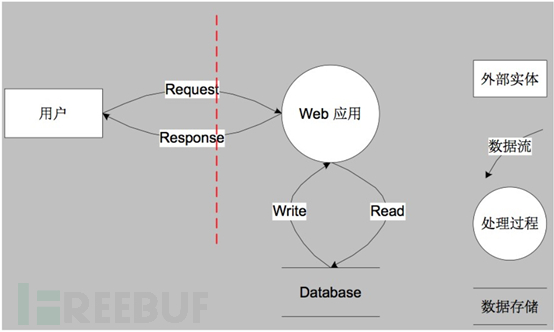
\includegraphics[scale=0.6]{resources/img/i5.png}
%     \caption{简单数据流图实例}
%   \end{figure}


\subsubsection{STRIDE四类元素与六类威胁的对应关系}

具体的对应关系2.4示例,并不是每个元素都会面临6个威胁,比如外部实体只有仿冒和抵赖两类威胁,我们不用关心外部实体会不会被篡改、会不会发生信息泄露、以及拒绝服务等,因为外部实体本来就是我们控制范围之外的。
其中进程(处理过程)会面临全部的6个威胁,数据存储中Repudiation(抵赖)是红色,表示只有存储的数据是审计类日志才会有抵赖的风险。
\begin{figure}
    \centering
    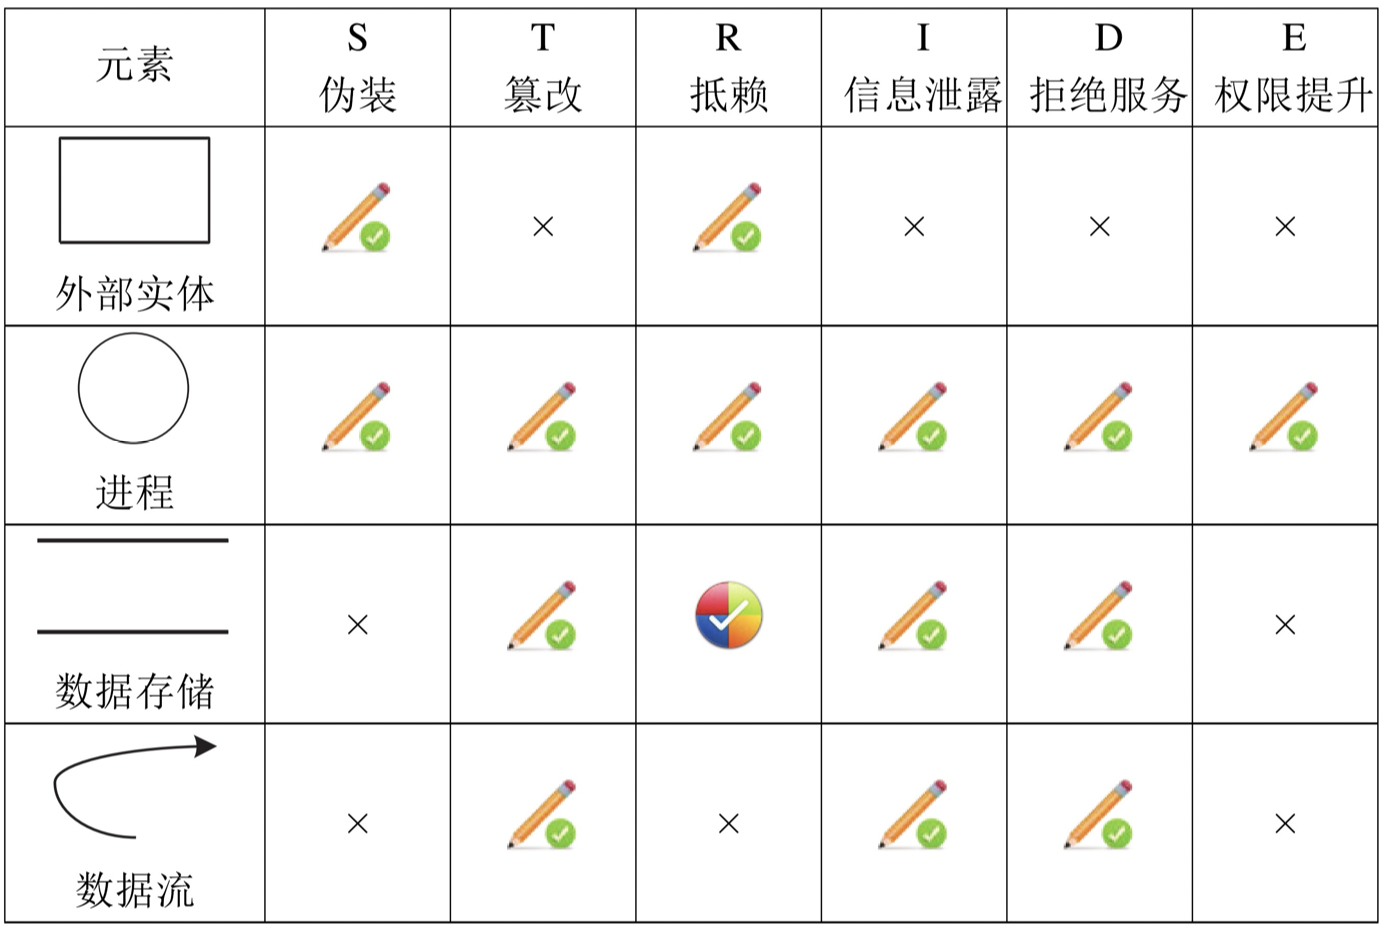
\includegraphics[scale=0.6]{resources/img/i77.png}
    \caption{四类元素和六类威胁对应关系}
  \end{figure}

\subsubsection{STRIDE 威胁建模流程}
(1) 分解业务场景,绘制数据流图表(DFD),以特定的场景为目标,
因此,应当按照实际的应用情况,如电商业务中采购、登记等进行分类。如果有
有多少种情况,或者如何划分,取决于用户所用的系统和企业。淘宝,京
与电商平台如拼多多、 AmazonEC2、腾讯等国产平台。不同的系统会产生不同的商业场景。每个服务与每个场景
STRIDE威胁建模是独立的,不会互相干扰,所以每个已分解的业务场景都要进行深入的研究,
对不同的 STRIDE威胁进行建模。接下来,就是要画出一个数据流图表。数据流图
四个单元:数据流(箭头)、数据存储单元(双横线)、进程(圆形)以及外部实体/交互方(正方
素数的标准符号。在图2.5中可以看到。
除以上四大核心部件之外,在实践中,还可以添加一个叫做“信任边界”的元素,我们用虚线标出的该元素。当数据流通过不同的信任界限时,就必须使用
用线条来区别信任边界。因为在接下来的威胁模型中,信任边界是不会被划分
所以,大部分的核心要素都包含:四大元素:进程,数据存储,数据流,以及交互方/外部实体
这里没有所谓的“信任边界”。在增加了信任边界之后,每个节点和每个数据流都必须执行分析
对其在6个维度的安全威胁进行分析和判定。

\begin{figure}
    \centering
    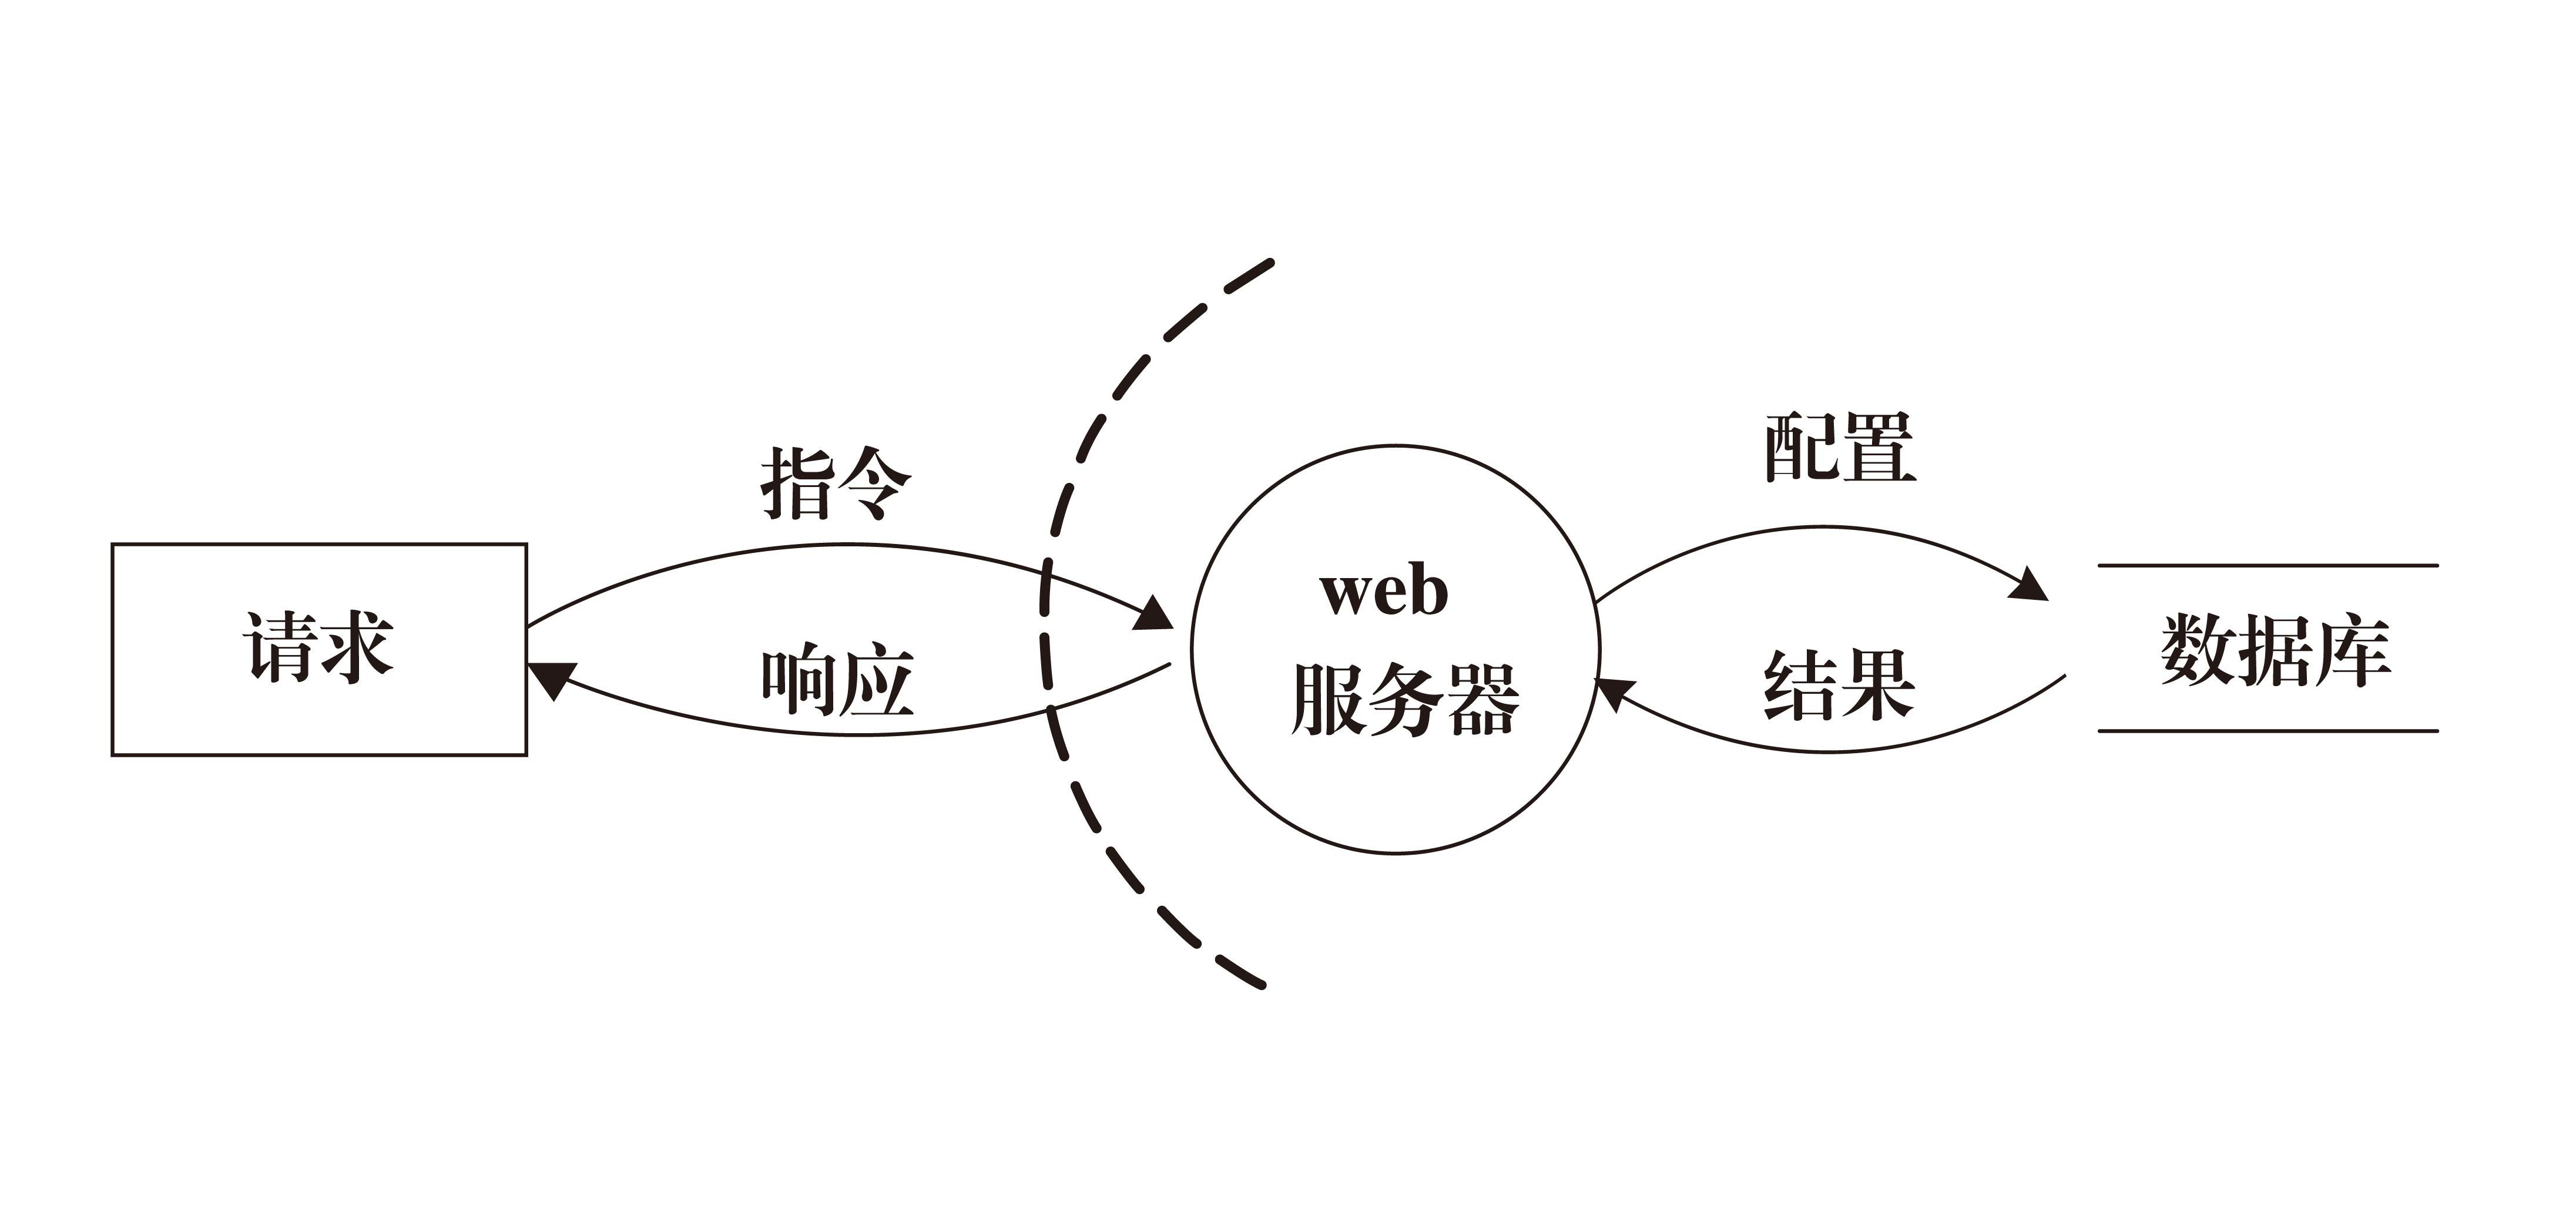
\includegraphics[scale=0.4]{resources/img/i7.jpg}
    \caption{常用web场景数据流图}
  \end{figure}
  (2)列出节点元素的安全威胁,逐个具体分析。绘制完数据流图之后,需要列
  出数据流中的每个节点元素可能面临的安全威胁,并逐个分析。如表 2.1 所示。

  表中列出了每种元素可能面临的安全威胁,下面对表进行简单分析数据流需要分析“篡改(替换)、外部实体可能面临“伪装”和
  “抵赖”两种威胁、“信息丢失或泄露”和“拒绝服务”三种威胁。

  \begin{table}
    \caption{元素STRIDE威胁分析}
  \begin{center}
    \begin{tabular}{|l|l|l|l|l|l|l}
      \hline 元素类型 & 伪装 & 篡改 & 抵赖 & 信息泄露 & 拒绝服务 & 权限提升\\
      \hline 外部实体 & X & X & X & X & X & X \\
      \hline 进程 & X & X & X & X & X & X \\
      \hline 数据存储 & X & X & X & X & X & X \\
      \hline 数据流 & X & X & X & X & X & X \\
      \hline
      \end{tabular}
  \end{center}
\end{table}
  (3)输出威胁列表:分析完数据流图中所有元素的潜在安全威胁后,如表2.2是一个输出威胁列表:包括消减方案和威胁评级。威胁列表可以帮助生成我们对威胁进行深入分析和改进的模型。
\begin{table}
  \caption{威胁列表}
\begin{center}
  \begin{tabular}{|l|l|}
    \hline 组件(威胁的目标) & GPS自动导航进程 \\
    \hline 威胁描述 & 黑客通过劫持GPS信号误导用户自动导航 \\
    \hline 威胁类别 & I \\
    \hline 攻击方法 & 利用网络监控劫持信号通道 \\
    \hline 消减方案(对策) & 提供加密和验证通道 \\
    \hline 危险评级 & 待定 \\
    \hline
    \end{tabular}
\end{center}
\end{table}
威胁等级,基于所产生的后果来评估和评分。这样就能对威胁进行归类,
首先要处理的是最大的威胁,其次才是较小的。学术上目前有很多种不同的威胁等级。
以安全缺陷等级为例,它包括 DREAD和 CVSS (Common Vulnerability Scoring System)
两种常见评级方法。不同的评估方式在维度和计算上存在细微差
不同,但从本质上讲,危险等级=发生的几率×所造成的损失。具体要根据实际用途使用。

DREAD 即 Damage Potential(潜在损失)Reproducibility(重现性);Exploitability(可利用性)Affected users(影
响的用户)Discoverability(被发现性)。最终的威胁评级由这 6 个指标加权平均计算得出,公式如下:

$$
\operatorname{Rank}[0: 10]=\frac{(D a m+\operatorname{Rep}+\operatorname{Exp}+A f f+\text { Dis })}{2}
$$

Rank代表着威胁等级,从0到10,代表着从零到高的危险。这一公式并非统一不变的标准,只是为了让该评级方式的威胁值与 CVSS范围保持相同。
每个指标的得分为0至4,表明了威胁的严重性。

\begin{table}
  \caption{威胁评级}
\begin{center}
  \begin{tabular}{|l|l|l|l|l|}
    \hline 等级 & 极高(4) & 高(3) & 中(2) & 低(1) \\
    \hline 潜在的损失D & 获取最高权限 & 泄露关键信息 & 泄露敏感信息 & 泄露其他信息 \\
    \hline 重现性R & 可随时攻击 & 易重复攻击 & 可重复攻击 & 难重复攻击 \\
    \hline 可利用性E & 非常容易利用 & 较为容易攻击 & 高级黑客可利用 & 攻击条件苛刻 \\
    \hline 受影响用户A & 所有用户 & 管理员 & 一般用户 & 其他用户 \\
    \hline 可发现性D & 漏洞过于明显 & 需要漏洞挖掘 & 限定范围可发现 & 隐藏性极高 \\
    \hline
    \end{tabular}
\end{center}
\end{table}

\subsection{攻击树模型}
在攻击树的树状构造中,以树状的形式表现出对系统的袭击,以以对象为根结点,以不同的方法完成此目标。在兄弟结点之间可以体现出某种进攻的逻辑,
见图2.6。“或(OR)”的关联代表任何一个子结点的方式,只有当它的父结点被执行时,
它的父结点就可以达到它的攻击目的;“与(AND)”是指在实现了全部的子结点后,对父结点进行了进攻;“顺序(SAND)”的关联是指在完成了所有的子结点后,完成了对父结点的进攻。
每个攻击树的路径代表一种
进攻计划的基础线路,其深度表示了攻击路径的难易程度。
在建立了一棵攻击树之后,可以对每个叶子节点进行数值的分配,并进行相应的计算。当一个数值被指定后,安全目标就可以被计算出来。
攻击属性可以帮助你把危险和攻击结合在一起。
攻击者可以把攻击者视为一种包含必要的知识或装备、完成一步所需要的时间、以及攻击者所要承受的物理和法律上的风险。
攻击树上的每一个结点的价值都可以作为运行和发展的成本。该攻击树为设计与需求决策提供了有力的支撑。如果攻击的代价大于收益
也就是说,很有可能不会有袭击。但是,当攻击者发现可以获得的利益时,就会进行攻击,从而要求我们进行防御措施。

\begin{figure}
    \centering
    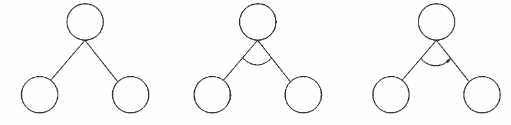
\includegraphics[scale=0.6]{resources/img/i8.png}
    \caption{攻击树基本结构}
  \end{figure}



  \section{层次分析法和FAHP}
  这里我们介绍下层次分析法用于第四章进行新的安全模型的理论基础。
  AHP 是一种结合定性和定量分析的多目标决策分析方
法,由萨蒂在20世纪70年代提出\cite{saaty1990make}。这种方法的主
要思想是通过将复杂的问题分解成几个层次来比较每两
个决策元素的相对重要性,每个层次由有限数量的决策
元素组成。然后建立满足性质(2)(3)的判断矩阵。通过
计算判断矩阵的最大特征值和相应的特征向量,从两两
比较中间接评估不同元素的相对重要性。层次分析法的
特点是将人们的主观判断数学化,使决策更容易被接
受。AHP 的过程可分为以下步骤:
\begin{itemize}
  \item  构建一个问题的层次结构,包括一个目标、实现
  目标的要素以及对这些要素进行评分的评估标
  准。
  \item  将决策元素成对比较,根据标度准则确定相对
  重要性,然后构造一个判断。
  \item  计算每个元素的权重并检查判断矩阵的一致
  性。
  \item 通过比较综合重要性,根据所有备选方案的优先
  级做出最终决策。
\end{itemize}

然而,层次分析法难以检查判断矩阵的一致性,其一
致性判断准则缺乏科学依据。此外,当有许多评价指标
时,很难保证决策的一致性。在这种情况下,FAHP 应运而
生\cite{min1997fuzzy}。一种是基于模糊数的 FAHP,另一种是基于模糊判
断矩阵的。FAHP 的过程与层次分析法相同,但仍有两个
不同之处:
\begin{itemize}
  \item  建立的判断矩阵不同:层次分析法是判断矩阵,而
  FAHP 是模糊判断矩阵
  判断矩阵。
  \item  寻找矩阵中每个元素相对重要性的不同加权方
  法。
\end{itemize}


\section{本章小结}

本章主要介绍了智能网联汽车的系统架构,首先从整体上给出其车联网系
统的架构介绍,然后对 TSP 云服务、V2X,车载网络通信进行了详细分
析,解释了车载网络通信各个协议之前的区别和优劣。
然后介绍了三种类型的威胁方面。最后主要介绍智能网联汽车领域的威胁建模分析:
首先介绍传统的 STRIDE 模型,攻击树模型,此外还介绍了AHP和FAHP层次分析法用于定量分析。
为后文叙述系统架构中存在的攻击入口以及漏洞打下基础。
为后续的智能互联汽车威胁模型的提出提供了前置理论来源。